\documentclass[12pt]{beamer}
\newenvironment{ConCodigo}[1]
  {\begin{frame}[fragile,environment=ConCodigo]{#1}}
  {\end{frame}}
\graphicspath{{Imagenes/}{../Imagenes/}}
\usepackage[utf8]{inputenc}
\usepackage[spanish]{babel}
\usepackage{hyperref}
\usepackage{etex}
%\reserveinserts{28}
\usepackage{amsmath}
\usepackage{amsthm}
\usepackage{mathtools}
\usepackage{multicol}
\usepackage{multirow}
\usepackage{tabulary}
\usepackage{booktabs}
\usepackage{nccmath}
\usepackage{physics}
\usepackage{biblatex}
\usepackage[outdir=./]{epstopdf}
%\epstopdfsetup{outdir=./}
\usepackage{graphicx}
%\usepackage{enumitem,xcolor}
\usepackage{siunitx}
%\sisetup{scientific-notation=true}
%\usepackage{fontspec}
\usepackage{lmodern}
\usepackage{float}
\usepackage[format=hang, font=footnotesize, labelformat=parens]{caption}
\usepackage[autostyle,spanish=mexican]{csquotes}
\usepackage{standalone}
\usepackage{blkarray}
\usepackage{algorithm}
\usepackage{algorithmic}
\usepackage{tikz}
\usepackage[siunitx, RPvoltages]{circuitikz}
\usetikzlibrary{arrows,patterns,shapes}
\usetikzlibrary{decorations.markings}
\usetikzlibrary{arrows}
\usepackage{color}
\usepackage{xcolor}
%\usepackage{beton}
%\usepackage{euler}
%\usepackage[T1]{fontenc}
\usepackage[sfdefault]{roboto}  %% Option 'sfdefault' only if the base font of the document is to be sans serif
\usepackage[T1]{fontenc}
\renewcommand*\familydefault{\sfdefault}
\DeclareGraphicsExtensions{.pdf,.png,.jpg}
\usepackage{hyperref}
\renewcommand {\arraystretch}{1.5}
\newcommand{\python}{\texttt{python}}
\usefonttheme[onlymath]{serif}
\setbeamertemplate{navigation symbols}{}
\usetikzlibrary{patterns}
\usetikzlibrary{decorations.markings}
\tikzstyle{every picture}+=[remember picture,baseline]
%\tikzstyle{every node}+=[inner sep=0pt,anchor=base,
%minimum width=2.2cm,align=center,text depth=.15ex,outer sep=1.5pt]
%\tikzstyle{every path}+=[thick, rounded corners]
\setbeamertemplate{caption}[numbered]
\newcommand{\ptm}{\fontfamily{ptm}\selectfont}
%Se usa la plantilla Warsaw modificada con spruce
\mode<presentation>
{
  \usetheme{Warsaw}
  \setbeamertemplate{headline}{}
  \useoutertheme{default}
  \usecolortheme{albatross}
  \setbeamercovered{invisible}
}
% \AtBeginSection[]
% {
% \begin{frame}<beamer>{Contenido}
% \normalfont\mdseries
% \tableofcontents[currentsection]
% \end{frame}
% }

%Se usa la plantilla Warsaw modificada con spruce
\mode<presentation>
{
  \usetheme{Warsaw}
  \setbeamertemplate{headline}{}
  %\useoutertheme{infolines}
  \usecolortheme{crane}
  \setbeamercovered{invisible}
  

\setbeamertemplate{section in toc}[sections numbered]
\setbeamertemplate{subsection in toc}[subsections numbered]
\setbeamertemplate{subsection in toc}{\leavevmode\leftskip=3.2em\rlap{\hskip-2em\inserttocsectionnumber.\inserttocsubsectionnumber}\inserttocsubsection\par}
\setbeamercolor{section in toc}{fg=blue}
\setbeamercolor{subsection in toc}{fg=blue}
\setbeamerfont{subsection in toc}{size=\small}



\setbeamertemplate{navigation symbols}{}
\setbeamertemplate{caption}[numbered]
% \setbeamercolor{frametitle}{fg=yellow,bg=blue!70!white}
%\setbeamercolor{section in head}{bg=green,fg=white}
%\setbeamercolor{subsection in head/foot}{bg=gray!30,fg=black}
%\setbeamercolor{author in head/foot}{fg=yellow}
%\setbeamercolor{date in head/foot}{fg=blue}

%\mode<presentation>
%{
%  \usetheme{Warsaw}
%  \setbeamertemplate{headline}{}
%  %\useoutertheme{infolines}
%  \useoutertheme{default}
%  \setbeamercovered{invisible}
%  % or whatever (possibly just delete it)
%}
}

\input{../Preambulos/pre_codigo}
\makeatletter
%\setbeamercolor{section in foot}{bg=gray!30, fg=black!90!orange}
%\setbeamercolor{subsection in foot}{bg=blue!30!yellow, fg=red}
\setbeamertemplate{footline}
{
  \leavevmode%
  \hbox{%
  \begin{beamercolorbox}[wd=.333333\paperwidth,ht=2.25ex,dp=1ex,center]{author in foot}%
    \usebeamerfont{author in head/foot} \textcolor{red}{\insertsection}
  \end{beamercolorbox}}%
  \begin{beamercolorbox}[wd=.333333\paperwidth,ht=2.25ex,dp=1ex,center]{title in foot}%
    \usebeamerfont{title in head/foot}\insertsubsection
  \end{beamercolorbox}%
  \begin{beamercolorbox}[wd=.333333\paperwidth,ht=2.25ex,dp=1ex,right]{date in head/foot}%
    \usebeamerfont{date in head/foot} \insertshortdate{} \hspace*{2em}
    \insertframenumber{} / \inserttotalframenumber \hspace*{2ex} 
  \end{beamercolorbox}}%
  \vskip0pt%
\makeatother	
\setbeamercolor{block title example}{use=structure, fg=white}
\normalfont
\usepackage{ccfonts}% http://ctan.org/pkg/{ccfonts}
\usepackage[T1]{fontenc}% http://ctan.or/pkg/fontenc
\renewcommand{\rmdefault}{cmr}% cmr = Computer Modern Roman
\linespread{1.3}
\title{Métodos numéricos para matrices}
\subtitle{Curso de Física Computacional}
\author{M. en C. Gustavo Contreras Mayén}
\date{}
\institute{Facultad de Ciencias - UNAM}
\titlegraphic{\includegraphics[width=1.75cm]{Imagenes/escudo-facultad-ciencias}\hspace*{4.75cm}~%
   \includegraphics[width=1.75cm]{Imagenes/escudo-unam}
}
\begin{document}
\maketitle
\fontsize{14}{14}\selectfont
\spanishdecimal{.}
\section*{Contenido}
\frame[allowframebreaks]{\tableofcontents[currentsection, hideallsubsections]}
\section{Introducción}
\frame{\tableofcontents[currentsection, hideothersubsections]}
\subsection{Primer ejemplo: Vibraciones en una molécula}
\begin{frame}
\frametitle{Primer ejemplo: Vibraciones en una molécula}
Supongamos que queremos estudiar el espectro de vibraciones de una molécula con $n$ grados de libertad.
\end{frame}
\begin{frame}
\frametitle{Primera aproximación}
La primera aproximación consiste en investigar las oscilaciones armónicas del sistema, expandiendo la energía potencial hasta el segundo orden en las coordenadas generalizadas alrededor de las posiciones de equilibrio:
\pause
\begin{align*}
U(q_{1}, q_{2}, \ldots, q_{n}) \simeq \dfrac{1}{2} \sum_{i, j = 1} A_{i j} \: q_{i} \: q_{j}
\end{align*}
\end{frame}
\begin{frame}
\frametitle{Energía potencial}
\begin{align*}
U(q_{1}, q_{2}, \ldots, q_{n}) \simeq \dfrac{1}{2} \sum_{i, j = 1} A_{i j} \: q_{i} \: q_{j}
\end{align*}
donde $q_{i}$ son las coordenadas generalizadas y $A_{j k}$ son parámetros del potencial que usualmente pueden obtenerse a partir de un cálculo de química cuántica.
\end{frame}
\begin{frame}
\frametitle{Energía cinética}
La energía cinética puede escribirse en términos de las velocidades generalizadas:
\begin{align*}
T(\dot{q_{1}}, \dot{q_{2}}, \ldots, \dot{q_{n}}) \simeq \dfrac{1}{2} \sum_{i, j=1} M_{i j} \: \dot{q_{i}} \: \dot{q_{j}}
\end{align*}
donde las $\dot{q}_{i}= \dv*{q_{i}}{t}$ son las velocidades generalizadas, las $M_{i j}$ son los elementos de masa generalizado en la matriz, cuyos valores dependen en particular de la molécula. 
\end{frame}
\begin{frame}
\frametitle{El Lagrangiano}
Aplicando la ecuación de Lagrange
\begin{align*}
\pdv{\mathcal{L}}{q_i} - \dv{t} \: \pdv{\mathcal{L}}{\dot{q_{i}}} = 0
\end{align*}
donde el Lagrangiano del sistema es: $\mathcal{L} = T - U$, por tanto, tenemos que:
\begin{align*}
\sum_{j = 1}^{n} \left( A_{ij} \: q_{j} + M_{ij} \: \ddot{q_{j}} \right) = 0, \hspace{1cm} i = 1, 2, \ldots, n
\end{align*}
\end{frame}
\begin{frame}
\frametitle{Dependencia del tiempo de tipo oscilatorio }
Si suponemos que la dependencia del tiempo en las coordenadas generalizadas es de tipo oscilatorio, con
\begin{align*}
q_{j} = x_{j} \: e^{-i \omega t}
\end{align*}
\pause
Se obtiene el siguiente sistema de ecuaciones homogéneo:
\begin{align*}
\sum_{j = 1}^{n} \left( A_{i j} -  \omega^{2} \: M_{i j} \right) x_{j} = 0, \hspace{1cm} i = 1, 2, \ldots, n
\end{align*}
\end{frame}
\begin{frame}
\frametitle{Expresión matricial}
La ecuación anterior se puede re-escribir en forma matricial, como.
\begin{align*}
\begin{pmatrix}
A_{11} & \ldots & A_{1n} \\
\vdots & \vdots & \vdots \\
A_{n1} & \ldots & A_{nn}
\end{pmatrix}
\begin{pmatrix}
x_{1} \\
\vdots \\
x_{n}
\end{pmatrix} = \lambda
\begin{pmatrix}
M_{11} & \ldots & M_{1n} \\
\vdots & \vdots & \vdots \\
M_{n1} & \ldots & M_{nn}
\end{pmatrix}
\begin{pmatrix}
x_{1} \\
\vdots \\
x_{n}
\end{pmatrix}
\end{align*}
\end{frame}
\begin{frame}
\frametitle{Expresión reducida}
De manera equivalente en una expresión reducida tenemos que:
\begin{align*}
\mathbf{A \: x} = \lambda \: \mathbf{M \: x}
\end{align*}
donde $\lambda= \omega^{2}$ es el valor propio y $\mathbf{x}$ es el correspondiente vector propio de la ecuación de valores propios.\\
\end{frame}
\begin{frame}
\frametitle{Solución no trivial del sistema}
Este es un sistema de ecuaciones lineales homogéneas; con el fin de contar con una solución no trivial del conjunto de ecuaciones (que todos los componentes sean cero), el determinante de la matriz de coeficientes debe anularse, esto es
\begin{align*}
det \, \abs{ \mathbf{A} - \lambda \: \mathbf{M} }= 0
\end{align*}
\end{frame}
\begin{frame}
\frametitle{Raíces de la ecuación matricial}
\begin{align*}
det \, \abs{ \mathbf{A} - \lambda \: \mathbf{M} }= 0
\end{align*}
Las raíces de esta ecuación: $\lambda_{k}$ con $k = 1, 2, \ldots, n$ proporcionan todas las frecuencias angulares vibracionales de la molécula
\begin{align*}
\omega_{k} = \sqrt{\lambda_{k}}
\end{align*}
\end{frame}
\subsection{Segundo ejemplo: Circuito eléctrico}
\begin{frame}[fragile]
\frametitle{Segundo ejemplo: Circuito eléctrico}
Consideremos el siguiente circuito eléctrico conocido como el \emph{puente de Wheastone}:
\begin{figure}
	\centering
	\includestandalone{Figuras/circuito_electrico_01}
\end{figure}
\end{frame}
\begin{frame}
\frametitle{Solución para el circuito}
Usamos las leyes de Kirchhoff en las mallas del circuito para obtener un conjunto de ecuaciones que relacionan los voltajes y las corrientes del circuito, luego entonces, resolverlo y encontrar las incógnitas.
\end{frame}
\begin{frame}
\frametitle{Solución para el circuito}
Pero ahora veamos el caso del puente desbalanceado de Wheastone: tenemos tres circuitos (o mallas) independientes que marcaremos de color rojo y analizamos cada una de ellas:
\end{frame}
\begin{frame}[fragile]
\frametitle{Malla independiente 1}
\begin{figure}
	\centering
	\includestandalone{Figuras/circuito_electrico_02}
\end{figure}
\begin{align*}
r_{s} \: i_{1} + r_{1} \: i_{2} + r_{2} \: i_{3} = v_{0}
\end{align*}
\end{frame}
\begin{frame}[fragile]
\frametitle{Malla independiente 2}
\begin{figure}
	\centering
	\includestandalone{Figuras/circuito_electrico_03}
\end{figure}
\begin{align*}
-r_{x} \: i_{1} + ( r_{1} + r_{x} + r_{a}) \: i_{2} + r_{a} \: i_{3} = 0
\end{align*}
\end{frame}
\begin{frame}[fragile]
\frametitle{Malla independiente 3}
\begin{figure}
	\centering
	\includestandalone{Figuras/circuito_electrico_04}
\end{figure}
\begin{align*}
-r_{3} \: i_{1} - r_{a} \: i_{2} + ( r_{2} + r_{3} + r_{a}) \: i_{3} = 0
\end{align*}
\end{frame}
\begin{frame}
\frametitle{Sistema de ecuaciones}
Entonces tenemos un sistema de ecuaciones que resulta ser:
\begin{align*}
r_{s} \: i_{1} + r_{1} \: i_{2} + r_{2} \: i_{3} &= v_{0} \\
-r_{x} \: i_{1} + (r_{1} + r_{x} + r_{a}) \: i_{2} + r_{a} \: i_{3} &= 0 \\
-r_{3} \: i_{1} - r_{a} \: i_{2} + (r_{2} + r_{3} + r_{a}) \: i_{3} &= 0
\end{align*}
\pause
El sistema anterior se puede escribir como
\begin{align*}
\mathbf{R \: i} = \mathbf{v}
\end{align*}
\end{frame}
\begin{frame}
\frametitle{Descripción del sistema}
\begin{align*}
\mathbf{R \: i} = \mathbf{v}
\end{align*}
donde la matriz de coeficientes de las resistencias es
\begin{align*}
\mathbf{R} =
\begin{pmatrix}
r_{s} & r_{1} & r_{2} \\
-r_{x} & r_{1} + r_{x} + r_{a} & -r_{a} \\
-r_{3} & -r_{a} & r_{2} + r_{3} + r_{a}
\end{pmatrix}
\end{align*}
\end{frame}
\begin{frame}
\frametitle{Descripción del sistema}
Los vectores columna de corrientes y voltajes son:
\begin{align*}
\mathbf{i} =
\begin{pmatrix}
i_{1} \\
i_{2} \\
i_{3}
\end{pmatrix}
\hspace{2cm}
\mathbf{v} =
\begin{pmatrix}
v_{0} \\
0 \\
0
\end{pmatrix}
\end{align*}
\end{frame}
\begin{frame}
\frametitle{Solución del sistema matricial}
Multiplicando en ambos lados por $\mathbf{R}^{-1}$ (la matriz inversa de $\mathbf{R}$), la ecuación
\begin{align*}
\mathbf{Ri} = \mathbf{v}
\end{align*}
resulta
\begin{align*}
\mathbf{i} = \mathbf{R}^{-1}\mathbf{v}
\end{align*}
entoces se requiere que conozcamos $\mathbf{R}^{-1}$.
\\
\bigskip
\pause
¿Será necesario conocer siempre la matriz inversa?
\end{frame}
\section{Sistemas lineales algebraicos}
\frame[allowframebreaks]{\tableofcontents[currentsection, hideothersubsections]}
\subsection*{Sistemas lineales con la computadora}
\begin{frame}
\frametitle{Sistemas lineales algebraicos}
En este tema analizamos la solución numérica de sistemas de ecuaciones lineales algebraicos, con $n$ incógnitas.
\\
\bigskip
Nos apoyaremos en gran medida en lo que aprendimos en el curso de Álgebra Lineal 1 más elementos computacionales de \python, para simplificar el proceso de solución.
\end{frame}
\begin{frame}
\frametitle{Sistemas lineales algebraicos}
Cuando tomamos un problema físico, los conjuntos de ecuaciones a menudo son muy grandes, por lo que consumen una gran cantidad de recursos computacionales.
\\
\bigskip
Ya hemos mencionado que un sistema será \emph{grande}, cuando el tamaño sea igual o mayor a una matriz de $50 \cp 50$ 
\end{frame}
\subsection*{Uso de propiedades de la matriz}
\begin{frame}
\frametitle{Uso de propiedades de la matriz}
Por lo general, se reducen los requerimientos de almacenamiento y el tiempo de ejecución mediante el aprovechamiento de propiedades especiales de la matriz de coeficientes, tales como poca densidad (la mayoría de los elementos de un matriz dispersa son cero -las llamadas matrices \textit{sparse}-)
\end{frame}
\begin{frame}
\frametitle{Ejemplo matriz tipo \emph{sparse}}
\begin{align*}
A = \begin{pmatrix}
a_{11} & a_{12} & a_{13} & 0 & 0 & 0 & 0 \\
a_{21} & a_{22} & 0 & a_{24} & a_{25} & 0 & 0 \\
a_{31} & 0 & a_{33} & a_{34} & 0 & 0 & 0 \\
0 & a_{42} & a_{43} & a_{44} & 0 & a_{46} & 0 \\
0 & a_{52} & 0 & 0 & a_{55} & 0 & a_{57} \\
0 & 0 & 0 & a_{64} & 0 & a_{66} & a_{67} \\
0 & 0 & 0 & 0 & a_{75} & a_{76} & 0
\end{pmatrix}
\end{align*}
\end{frame}
\begin{frame}
\frametitle{De la matriz tipo \emph{sparse}}
La matriz $\mathbf{A}$ es una matriz dispersa de $7 \cp 7 = 49$ entradas.
\\
\bigskip
Definimos $\eta (\mathbf{A})$ el número de entradas no nulas de $\mathbf{A}$, entonces tenemos que $\eta (\mathbf{A}) = 22$.
\end{frame}
\begin{frame}
\frametitle{Otros tipos de matrices}
Es posible encontrar otros tipos de matrices, pero si visualizamos solo las entradas que son distintas de cero, tendremos una imagen del sistema que se nos presenta.
\\
\bigskip
Los puntos negros a continuación representan las entradas de la matriz no nulas.
\end{frame}
\begin{frame}
\frametitle{Matriz en banda}
\begin{figure}[h!]
    \centering
    \includegraphics[scale=0.6]{Imagenes/tipo_matrices_01_banda.png}
    \caption{Matriz en banda.}
\end{figure}
\end{frame}
\begin{frame}
\frametitle{Matriz no estructurada}
\begin{figure}[h!]
    \centering
    \includegraphics[scale=0.6]{Imagenes/tipo_matrices_02_no_estructurada.png}
    \caption{Matriz no estructurada.}
\end{figure}
\end{frame}
\begin{frame}
\frametitle{Matriz skyline}
\begin{figure}[h!]
    \centering
    \includegraphics[scale=0.6]{Imagenes/tipo_matrices_03_skyline.png}
    \caption{Matriz tipo skyline.}
\end{figure}
\end{frame}
\subsection{Algoritmos de solución}
\begin{frame}
\frametitle{Algoritmos específicos de solución}
Existen muchos algoritmos dedicados a la solución de grandes conjuntos de ecuaciones, cada uno de ellos está adaptado a una determinada forma del coeficiente de la matriz ya sea de tipo: simétrica, en bandas, \emph{sparse}, etc.)
\end{frame}
\subsection{Librerías de algoritmos}
\begin{frame}
\frametitle{Librerías de algoritmos}
En internet se encuentran disponibles librerías para resolver cierto tipo de problemas, al usarlas se requiere conocer la manera en que se proporcionan los argumentos y las variables de resultado que proporcionan, se obliga la revisión de la documentación de cada uno de los códigos.
\end{frame}
\begin{frame}
\frametitle{Librerías de algoritmos}
Toma en cuenta de que las librerías se \enquote{construyen} en un lenguaje de programación particular, no todo estará en el lenguaje de nuestra predilección.
\\
\bigskip
En la siguiente tabla se revisan algunas librerías, los lenguajes nativos y su disposición (libre o de pago)
\end{frame}
\begin{frame}[fragile]
\frametitle{Librerías de algoritmos}
\fontsize{12}{12}\selectfont
\begin{table}
\begin{tabular}{ p{4cm} p{3cm} l}
Librería & Lenguaje & Tipo de licencia \\ \hline
ATLAS & C & Libre \\ \hline
Dlib & \verb|C++| & Libre \\ \hline
GNU Scientific Library & C, \verb|C++| & Libre \\ \hline
IMSL & C, Java, \verb|C#|, Fortran, Python & De pago \\ \hline
LAPACK & Fortran & Libre \\ \hline
MKL & \verb|C++|, Fortran & De pago \\ \hline
Eigen & \verb|C++| & Libre \\ \hline
\end{tabular}
\end{table}
\end{frame}
\begin{frame}
\frametitle{Librerías de algoritmos}
No son las únicas librerías disponibles, son las más referidas y publicadas, ya en casos muy especiales, se pueden encontrar sitios donde se publican ya sea parcial o totalmente el contenido de las librerías.
\end{frame}
\subsection{Sistema algebraico}
\begin{frame}
\frametitle{Definición de sistema algebraico}
Ya revisamos en la presentación anterior lo que es un sistema algebraico:
\begin{align*}
A_{11} x_{1} + A_{12} x_{2} + \ldots + A_{1n} x_{n} &= b_{1} \\
A_{21} x_{1} + A_{22} x_{2} + \ldots + A_{2n} x_{n} &= b_{2} \\
 &= \vdots \\
A_{n1} x_{1} + A_{n2} x_{2} + \ldots + A_{nn} x_{n} &= b_{n} \\
\end{align*}
\pause
o sencillamente
\begin{align*}
\mathbf{A \: x} = \mathbf{b}
\end{align*}
\end{frame}
\begin{frame}[fragile]
\frametitle{Matriz aumentada}
Una representación particularmente útil de las ecuaciones para los propósitos computacionales es la \emph{matriz de coeficientes aumentada}, que se obtiene al juntar el vector constante $b$ a la matriz de coeficientes $A$ de la siguiente manera:
\end{frame}
\begin{frame}[fragile]
\frametitle{Matriz aumentada}
\begin{align*}
\qty[ A \vert b ] = 
\begin{bmatrix}[c c c c | c]
A_{11} & A_{12} & \ldots & A_{1n} & b_{1} \\
A_{21} & A_{22} & \ldots & A_{2n} & b_{2} \\
\vdots & \vdots & \ddots & \vdots & \vdots  \\
A_{n1} & A_{n2} & \ldots & A_{nn} & b_{n} 
\end{bmatrix}
\end{align*} 
\end{frame}
\subsection{Unicidad de la solución}
\begin{frame}
\frametitle{Unicidad de la solución}
Un sistema de $n$ ecuaciones lineales con $n$ incógnitas tiene una solución única, siempre que el determinante de la matriz de coeficientes sea \textcolor{red}{no singular}, es decir, $det \, \vert A \vert \neq 0$. 
\end{frame}
\begin{frame}
\frametitle{Unicidad de la solución}
Las filas y columnas de una matriz no singular son linealmente independientes en el sentido de que no hay ninguna fila (o columna) que sea una combinación lineal de las otras filas (o columnas)
\end{frame}
\begin{frame}
\frametitle{Soluciones infinitas}
Si la matriz de coeficientes es singular, las ecuaciones pueden tener un número infinito de soluciones o no soluciones en absoluto, dependiendo del vector constante.
\end{frame}
\subsection*{Caso 1: Soluciones infinitas}
\begin{frame}
\frametitle{Caso 1}
Como ejemplo veamos el sistema de ecuaciones:
\begin{align*}
2 \, x + y &= 3 \\
4 \,x + 2 \, y &= 6
\end{align*}
\pause
La segunda ecuación puede obtenerse multiplicando la primera ecuación por dos.
\end{frame}
\begin{frame}
\frametitle{Caso 1}
Cualquier combinación de $x$ e $y$ que satisface la primera ecuación es también una solución de la segunda.
\\
\bigskip
El número de tales combinaciones es infinito.
\end{frame}
\begin{frame}
\frametitle{Gráfica de las ecuaciones}
Si graficamos las ecuaciones tenemos que las dos rectas se superponen:
\begin{figure}
	\centering
	\includegraphics[scale=0.3]{Imagenes/Grafica01.eps}
	\caption{Representación gráfica cuando la matriz de coeficientes es singular.}
\end{figure}
\end{frame}
\subsection*{Caso 2: Sistemas sin solución}
\begin{frame}
\frametitle{Caso 2}
En otro caso, este sistema de ecuaciones:
\begin{align*}
2 \: x + y &= 3 \\
4 \: x + 2 \:y &= 0
\end{align*}
No tienen solución, ya que la ecuación equivalente $2 \: x + y = 0$, contradice la primera.
\\
\bigskip
\pause
Por tanto, cualquier solución que satisface la primera, no puede satisfacer la segunda.
\end{frame}
\begin{frame}
\frametitle{Gráfica del sisteama}
Al graficar tenemos que las dos rectas son paralelas
\begin{figure}
	\centering
	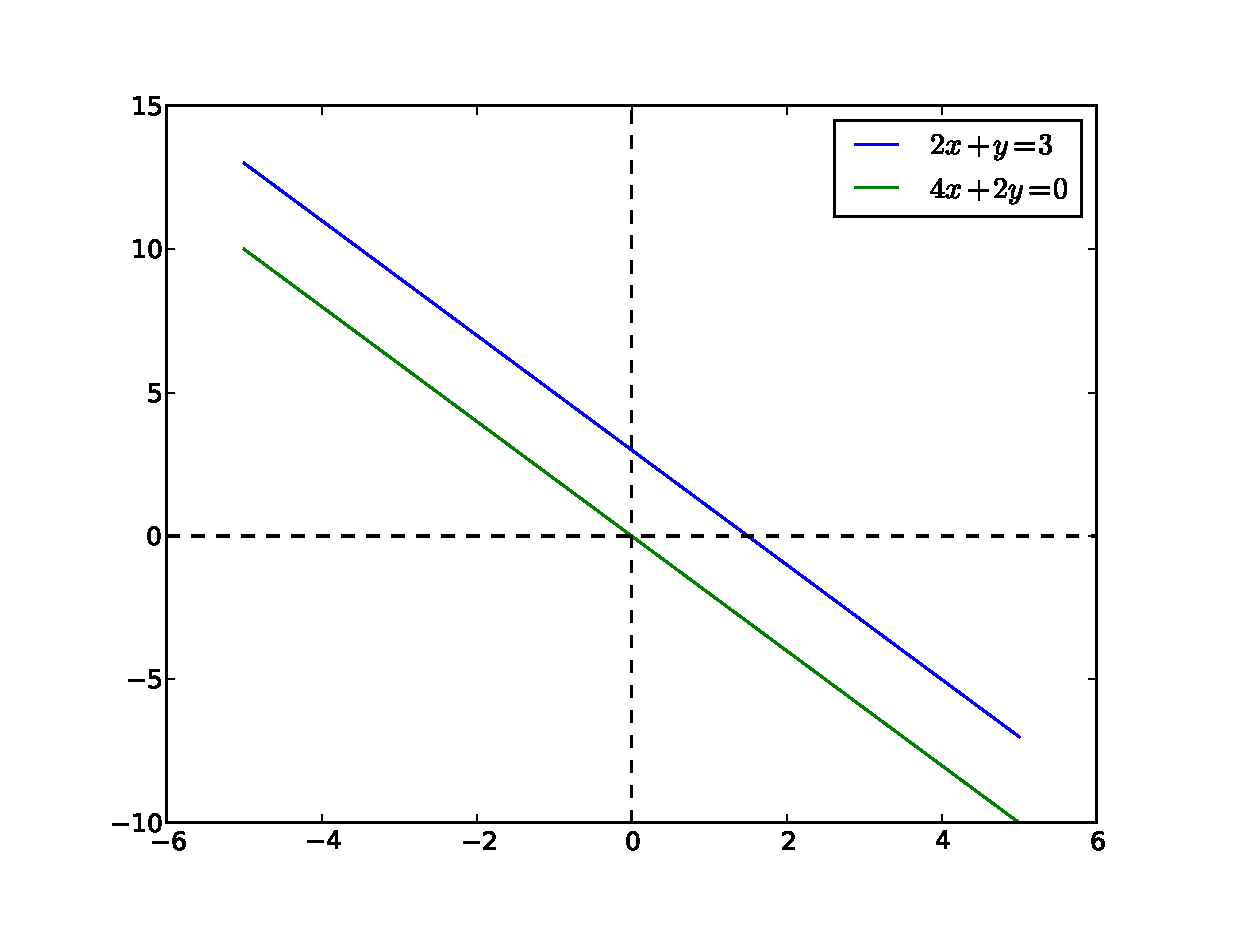
\includegraphics[scale=0.3]{Imagenes/Grafica02.eps}
	\caption{Representación gráfica de un sistema algebraico sin solución.}
\end{figure}
\end{frame}
\subsection{Problemas mal condicionados}
\begin{frame}
\frametitle{Problemas mal condicionados}
Una pregunta obvia es: ¿qué sucede cuando la matriz de coeficientes es casi singular? es decir, si el $det \, \vert A \vert$ es muy pequeño?
\end{frame}
\begin{frame}
\frametitle{Problemas mal condicionados}
Con el fin de concluir si el determinante de la matriz es pequeño, necesitamos una referencia contra la cual el determinante se pueda medir.
\end{frame}
\subsection*{Norma de una matriz}
\begin{frame}
\frametitle{Norma de una matriz}
Esta referencia se denomina la \funcionazul{norma} de la matriz y se denota por $\norm{A}$.
\\
\bigskip
\pause
Entonces podemos decir que el determinante de la matriz es pequeño si
\begin{align*}
\det \, \qty| A | \ll \norm{A}
\end{align*}
\end{frame}
\begin{frame}
\frametitle{Definición de la norma de una matriz}
Existen diferentes maneras de calcular la norma de una matriz, tales como
\begin{align*}
\norm{A} &= \sqrt{\sum_{i = 1}^{n} \: \sum_{j = 1}^{n} \:  A^{2}_{i j}} \\[1em]
\norm{A} &= \max  \limits_{1 \leq i \leq j} \sum_{j=1}^{n} \: \abs{A_{ij}}
\end{align*}
\end{frame}
\subsection{Número de condición de la matriz}
\begin{frame}
\frametitle{Número de condición de la matriz}
Una medida formal del condicionamiento de una martiz, está dada por el \funcionazul{número de condición} de la matriz, definido por:
\begin{align*}
\mbox{cond}(A) = \norm{A} \, \norm{A^{-1}}
\end{align*}
Si este número \emph{es cercano a la unidad}, la matriz \textbf{está bien condicionada}.
\end{frame}
\begin{frame}
\frametitle{Número de condición de la matriz}
El número de condición aumenta con el grado de mal acondicionamiento, tendiendo a infinito para una matriz singular.
\\
\bigskip
Toma en cuenta que el número de condición no es único, sino que depende de la elección de la norma de la matriz.
\end{frame}
\begin{frame}
\frametitle{Número de condición de la matriz}
Desafortunadamente, el número de condición es costoso de calcular para grandes matrices.
\\
\bigskip
En la mayoría de los casos es suficiente para medir el condicionamiento comparando el determinante con las magnitudes de los elementos en la matriz.
\end{frame}
\subsection*{Efectos del mal condicionamiento}
\begin{frame}
\frametitle{Efectos del mal condicionamiento}
Si las ecuaciones están mal condicionadas, pequeños cambios en la matriz de coeficientes dan como resultado grandes cambios en la solución.
\end{frame}
\begin{frame}
\frametitle{Efectos del mal condicionamiento}
A modo de ejemplo, consideremos las ecuaciones:
\begin{align*}
2 \: x + y &= 3 \\
2 \: x + 1.001 \:y &= 0
\end{align*}
que tiene la solución $x = 1501.5$, $y = -3000$
\end{frame}
\begin{frame}[fragile]
\frametitle{La norma es menor que los coeficientes}
Dado que el determinante 
\begin{align*}
\abs{A} = 2 \: (1.001) - 2 \: (1) = 0.002 
\end{align*}
 es mucho menor que los coeficientes, las ecuaciones están mal condicionadas.
\\
\bigskip
\pause
Usemos \python{} para explorar este sistema de ecuaciones.
\end{frame}
\subsection*{Representación de las matrices}
\begin{frame}
\frametitle{Representación de las matrices}
El sistema de ecuaciones algebraicas
\begin{align*}
2 \: x + y &= 3 \\
2 \: x + 1.001 \:y &= 0
\end{align*}
Se va a representar de la siguiente forma:
\end{frame}
\begin{frame}
\frametitle{Matrices $\mathbf{A \: x =  b}$}
\begin{align*}
\mathbf{A} = \begin{pmatrix}
2 & 1 \\
2 & 1.001
\end{pmatrix}
\hspace{2cm}
\mathbf{b} = \begin{pmatrix}
3 \\
0
\end{pmatrix}
\end{align*}
\end{frame}
\begin{frame}[fragile]
\frametitle{Usando un \funcionazul{array}}    
\begin{align*}
\mathbf{A} = \begin{pmatrix}
2 & 1 \\
2 & 1.001
\end{pmatrix}
\end{align*}
\vspace{1cm}
\begin{verbatim}
A = np.array([[2., 1.], [2, 1.001]])
\end{verbatim}
\end{frame}
\begin{frame}[fragile]
\frametitle{Calculando el determinante}
Como lo vimos en la presentación pasada, usamos el paquete y librería \funcionazul{numpy.linalg} para estudiar el sistema
\begin{exampleblock}{Definimos las matrices}
\textcolor{ao}{\texttt{In[1]: }} \texttt{a = np.array([[2., 1.], [2, 1.001]])} \\
\medskip
\pause
\textcolor{ao}{\texttt{In[2]: }} \texttt{b = np.array([3., 0.])} \\
\medskip
\pause
\textcolor{ao}{\texttt{In[3]: }} \texttt{print (nla.det(a))} \\
\medskip
\pause
\textcolor{red}{\texttt{Out[3]: }} \texttt{0.002}
\end{exampleblock}
\end{frame}
\begin{frame}[fragile]
\frametitle{Número de condición}
Ahora calculamos el valor del número de condición	
\begin{exampleblock}{Cálculo del número de condición}
\textcolor{ao}{\texttt{In[4]: }} \texttt{print(nla.cond(a))} \\
\medskip
\pause
\textcolor{red}{\texttt{Out[4]: }} \texttt{5001.000300039825}
\end{exampleblock}
\end{frame}
\begin{frame}[fragile]
\frametitle{Solución del sistema}
Resolvemos el sistema algebraico
\begin{exampleblock}{Usamos la función \texttt{nla.solve}}
\textcolor{ao}{\texttt{In[5]: }} \texttt{print(nla.solve(a, b))} \\
\medskip
\pause
\textcolor{red}{\texttt{Out[5]: }} \texttt{[ 1501.5 -3000. ]}
\end{exampleblock}
\end{frame}
\begin{frame}[fragile]
\frametitle{El sistema está mal condicionado}
El efecto de los malos acondicionamientos se puede verificar mediante un pequeño cambio en la segunda ecuación:
\begin{align*}
2 \, x + y &= 3 \\
2 \, x + 1.002 \, y &= 0
\end{align*}
\end{frame}
\begin{frame}[fragile]
\frametitle{El sistema está mal condicionado}
Creamos un nuevo arreglo $c$ y calculamos el número de condición:
\begin{exampleblock}{Revisión del sistema con el cambio}
\textcolor{ao}{\texttt{In[6]: }} \texttt{c = np.array([[2.,1.],[2.,1.002]])} \\
\medskip
\pause
\textcolor{ao}{\texttt{In[7]: }} \texttt{print(nla.cond(c))} \\
\medskip
\pause
\textcolor{red}{\texttt{Out[7]: }} \texttt{2501.000600159942}
\end{exampleblock}
\end{frame}
\begin{frame}[fragile]
\frametitle{Resolvemos el sistema}
Usando la función \funcionazul{nla.solve(a, b)}, resolvemos el sistema
\begin{exampleblock}{Solución al sistema algebraico}
\textcolor{ao}{\texttt{In[8]: }} \texttt{print(nla.solve(c, b))} \\
\medskip
\pause
\textcolor{red}{\texttt{Out[8]: }} \texttt{[  751.5 -1500. ]}
\end{exampleblock}
\end{frame}
\begin{frame}
\frametitle{\large{Un pequeño cambio provoca un enorme impacto}}
El resultado es $x = 751.5$, $y = -1500$.
\\
\bigskip
Nótese que un cambio del $0.1\%$ en el coeficiente de $y$ produce un cambio de $100\%$ en la solución!
\end{frame}
\section{Sistemas algebraicos lineales}
\frame[allowframebreaks]{\tableofcontents[currentsection, hideothersubsections]}
\subsection{Definiciones}
\begin{frame}
\frametitle{Sistemas algebraicos lineales}
Las ecuaciones algebraicas lineales, se presentan en casi todas las ramas del análisis numérico. 
\\
\bigskip
Su aplicación más visible es en el análisis de sistemas lineales: cualquier sistema cuya respuesta es proporcional a la entrada se considera que es lineal.
\end{frame}
\begin{frame}
\frametitle{Sistemas algebraicos lineales}
Los sistemas lineales incluyen estructuras, sólidos, elásticos, flujo de calor, filtraciones de líquidos, campos electromagnéticos, los circuitos eléctricos, etc. 
\\
\bigskip
Si el sistema es discreto, tal como una viga o un circuito eléctrico, entonces su análisis conduce directamente a ecuaciones algebraicas lineales.
\end{frame}
\subsection*{Sistemas algebraicos discretos}
\begin{frame}
\frametitle{Sistemas algebraicos discretos}
Si el sistema es discreto, como en los esfuerzos en una viga o circuito eléctrico, entonces su análisis conduce directamente a ecuaciones algebraicas lineales.
\end{frame}
\begin{frame}
\frametitle{Sistemas algebraicos discretos}
En el caso de una viga estática, por ejemplo, las ecuaciones surgen cuando se describen las condiciones de equilibrio de los soportes.
\\
\bigskip
Las incógnitas $x_{1}, x_{2}, \ldots, x_{n}$ representas las fuerzas en las uniones y las reacciones de soporte, mientras que las constantes $b_{1}, b_{2}, \ldots, b_{n}$ son las cargas externas.    
\end{frame}
\begin{frame}
\frametitle{Cambio a un sistema discreto}
El comportamiento de los sistemas continuos se describen por ecuaciones diferenciales, en lugar de ecuaciones algebraicas.
\\
\bigskip
Sin embargo, como el análisis numérico sólo puede ocuparse de variables discretas, es primero necesario aproximar una ecuación diferencial con un sistema de ecuaciones algebraicas.
\end{frame}
\subsection{Métodos conocidos de solución}
\begin{frame}
\frametitle{Métodos conocidos de solución}
Son conocidos los métodos de diferencias finitas, elementos finitos y métodos de contorno del elemento para el análisis de esta manera.
\end{frame}
\begin{frame}
\frametitle{Métodos conocidos de solución}
Estos métodos utilizan diferentes aproximaciones para conseguir una \textit{discretización}, pero en cada caso la tarea final es el mismo: resolver un sistema (a menudo un sistema muy grande) de ecuaciones lineales algebraicas.
\end{frame}
\subsection*{Expresiones de los sistemas algebraicos}
\begin{frame}
\frametitle{Expresiones de los sistemas algebraicos}
El modelado de sistemas lineales invariablemente da lugar a las ecuaciones de la forma $\mathbf{A \:x} = \mathbf{b}$, donde $\mathbf{b}$ es la entrada y $\mathbf{x}$ representa la respuesta del sistema.
\\
\bigskip
El coeficiente de la matriz $\mathbf{A}$, refleja las características del sistema, es independiente
de la entrada.
\end{frame}
\begin{frame}
\frametitle{Expresiones de los sistemas algebraicos}
En otras palabras, si se cambia la entrada, las ecuaciones tienen que ser resueltas de nuevo con una $\mathbf{b}$ diferente, pero el mismo $\mathbf{A}$. 
\\
\bigskip
Por lo tanto, es deseable tener un algoritmo que resuelva a ecuación la solución de algoritmo que puede gestionar cualquier número de vectores constantes con un mínimo esfuerzo computacional.
\end{frame}
\section{Métodos de solución}
\frame[allowframebreaks]{\tableofcontents[currentsection, hideothersubsections]}
\subsection{Solución directa o indirecta}
\begin{frame}
\frametitle{Métodos de solución}
Hay dos clases de métodos para resolver sistemas de ecuaciones lineales algebraicas:
\setbeamercolor{item projected}{bg=red!70!black,fg=white}
\setbeamertemplate{enumerate items}[circle]
\begin{enumerate}[<+->]	
\item Métodos directos.
\item Métodos indirectos.
\end{enumerate}
\end{frame}
\subsection{Métodos directos}
\begin{frame}
\frametitle{Métodos directos}
La característica común de los métodos directos es que transforman las ecuaciones originales en ecuaciones equivalentes (ecuaciones que tienen la misma solución) que se pueden resolver más fácilmente.
\end{frame}
\subsection*{Operaciones elementales}
\begin{frame}
\frametitle{Operaciones elementales}
La transformación se lleva a cabo por la aplicación de las tres operaciones citadas a continuación. 
\\
\bigskip
Estas \emph{operaciones elementales} no cambian la solución, pero pueden afectar el determinante de la matriz de coeficientes como se indica en el paréntesis.
\end{frame}
\begin{frame}
\frametitle{Operaciones elementales}
\setbeamercolor{item projected}{bg=red!70!black,fg=white}
\setbeamertemplate{enumerate items}[circle]
\begin{enumerate}[<+->]
\item Intercambiar dos ecuaciones (cambia el signo de $\vert A \vert$)
\item Multiplicar una ecuación por una constante distinta de cero (se multiplica $\vert A \vert$ por la misma constante)
\item Multiplicar una ecuación por una constante distinta de cero y luego restarlo de otra ecuación (deja a $\vert A \vert$ sin cambios)
\end{enumerate}
\end{frame}
\subsection{Métodos indirectos}
\begin{frame}
\frametitle{Métodos indirectos}
Los métodos iterativos, o métodos indirectos, comienzan con una suposición de la solución $x$, y luego repetidamente refinan la solución hasta alcanzar un criterio de convergencia.
\end{frame}
\begin{frame}
\frametitle{Métodos indirectos}
Los métodos iterativos son generalmente menos eficientes que sus homólogos directos debido al gran número de iteraciones necesarias.
\\
\bigskip
Pero sí tienen ventajas computacionales importantes si la matriz de coeficientes es muy grande y escasamente pobladas (la mayoría de los coeficientes son cero).
\end{frame}
\section{Tres métodos directos}
\frame[allowframebreaks]{\tableofcontents[currentsection, hideothersubsections]}
\subsection{Uso de matrices \texorpdfstring{$U$}{}, \texorpdfstring{$L$}{}, \texorpdfstring{$I$}{}}
\begin{frame}
\frametitle{Tres métodos directos}
A continuación se enumeran los tres métodos directos más usados, cada uno de los cuales utiliza operaciones elementales para producir su propia manera de resolver ecuaciones.
\end{frame}
\begin{frame}
\frametitle{Tres métodos directos}
\fontsize{12}{12}\selectfont
\begin{tabular}{l l l}
Método & Forma inicial & Forma final \\ \hline
Eliminación de Gauss & $A \: x = b$ & $U\: x = c$ \\
Descomposición LU & $A \: x = b$ & $L\: U\: x = b$ \\
Eliminación Gauss-Jordan & $A \: x = b$ & $I \: x = c$
\end{tabular}
\\
\bigskip
\fontsize{14}{14}\selectfont
Donde $\mathbf{U}$ representa una matriz triangular superior, $\mathbf{L}$ es una matriz triangular inferior e $\mathbf{I}$ es la matriz identidad. 
\end{frame}
\begin{frame}
\frametitle{Tres métodos directos}
Una matriz cuadrada se llama triangular si contiene sólo elementos cero en un lado de la diagonal principal.
\end{frame}
\begin{frame}
\frametitle{Matriz $U$}
Como ejemplo: una matriz triangular superior $U$ de $3 \cp 3$  tiene la forma
\begin{align*}
U = \begin{bmatrix}
U_{11} & U_{12} & U_{13} \\
0 & U_{22} & U_{23} \\
0 & 0 & U_{33}
\end{bmatrix}
\end{align*}
\end{frame}
\begin{frame}
\frametitle{Matrices $L$}
Mientras que una matriz triangular inferior $L$ de $3 \cp 3$ es del tipo:
\begin{align*}
L = \begin{bmatrix}
L_{11} & 0 & 0 \\
L_{21} & L_{22} & 0 \\
L_{31} & L_{32} & L_{33}
\end{bmatrix}
\end{align*}
\end{frame}
\subsection*{Matrices triangulares}
\begin{frame}
\frametitle{Matrices triangulares}
Las matrices triangulares juegan un papel importante en el álgebra lineal, ya que simplifican muchos cálculos.
\end{frame}
\begin{frame}
\frametitle{Matrices triangulares}
Por ejemplo, consideremos la ecuación $L \: x = c$:
\begin{align*}
L_{11} \: x_{1} =& c_{1} \\
L_{21} \: x_{1} + L_{22} \: x_{2} =& c_{2} \\
L_{31} \: x_{1} + L_{32} \: x_{2} + L_{33} \: x_{3} =& c_{3} \\
\vdots
\end{align*}
\end{frame}
\begin{frame}
\frametitle{Matrices triangulares}
Si se resuelven las ecuaciones hacia delante, comenzando con la primera ecuación, los cálculos son muy fáciles, ya que cada ecuación contiene sólo una incógnita a la vez.
\end{frame}
\subsection*{Sustitución hacia adelante}
\begin{frame}
\frametitle{Sustitución hacia adelante}
La solución se obtiene haciendo:
\begin{align*}
x_{1} &= \dfrac{c_{1}}{L_{11}} \\
x_{2} &= \dfrac{(c_{2} - L_{21} \: x_{1})}{L_{22}} \\
x_{3} &= \dfrac{(c_{3} - L_{31} \: x_{1} - L_{32} \: x_{2})}{L_{33}} \\
\ldots
\end{align*}
Este procedimiento se conoce como \emph{sustitución hacia adelante}.
\end{frame}
\subsection*{Sustitución hacia atrás}
\begin{frame}
\frametitle{Sustitución hacia atrás}
De una manera similar la operación $U \: x = c$, se encuentra en el proceso de eliminación de Gauss, y puede resolverse fácilmente por sustitución hacia atrás, que se inicia con la última ecuación y va retrocediendo a través de las ecuaciones.
\end{frame}
\begin{frame}
\frametitle{Sustitución hacia atrás}
Las ecuaciones $L \: U \: x = b$, que están asociadas con la descomposición $L \: U$, también pueden resolverse rápidamente si las sustituimos con dos conjuntos de ecuaciones equivalentes: $L \: y = b$ y $U \: x = y$.
\end{frame}
\begin{frame}
\frametitle{Sustitución hacia atrás}
Ahora $L \: y = b$ se puede resolverse para $y$ por sustitución hacia delante, seguido de la solución de $U \: x = y$ por medio de la sustitución hacia atrás.
\end{frame}
\subsection*{Matriz identidad}
\begin{frame}
\frametitle{Operaciones con la matriz identidad}
Las ecuaciones $I \: x = c$, que se generan en la eliminación Gauss-Jordan, son equivalentes a $x = c$ (recordemos la identidad $I \: x = x$), de modo que $c$ es la solución.
\end{frame}
\section{Apoyo con scipy}
\frame[allowframebreaks]{\tableofcontents[currentsection, hideothersubsections]}
\subsection{El módulo scipy.linalg}
\begin{frame}
\frametitle{El módulo \funcionazul{scipy.linalg}}
El módulo \funcionazul{scipy.linalg} extiende las funciones que hemos mencionado anteriormente del módulo \funcionazul{numpy.linalg}.
\\
\bigskip
Entre otras cosas, incluye un conjunto de funciones para resolver problemas matriciales de una manera en particular.
\end{frame}
\begin{frame}
\frametitle{Funciones básicas en \funcionazul{scipy.linalg}}
\fontsize{12}{12}\selectfont
\begin{tabular}{l | m{7.5cm}}
Función & Descripción \\ \hline
\funcionazul{inv(a)} & Calcula la inversa de una matriz. \\ \hline
\funcionazul{solve(a, b)} & Resuelve el sistema $a \: x = b$, para una matriz $a$ cuadrada. \\ \hline
\funcionazul{solve\_banded} & Resuelve el sistema $a \: x = b$, donde $x$ es una matriz en banda. \\ \hline
\funcionazul{det(a)} & Calcula el determinante de una matriz. \\ \hline
\funcionazul{norm(a)} & Calcula la norma de una matriz.
\end{tabular}
\end{frame}
\begin{frame}[fragile]
\frametitle{Factorizaciones en \funcionazul{scipy.linalg}}
\fontsize{12}{12}\selectfont
\begin{tabular}{l | m{7.5cm}}
Función & Descripción \\ \hline
\funcionazul{lu(a)} & Factoriza $L \: U$ de una matriz $a$, devuleve la matriz pivote $P$, la matriz triangular inferior $L$ y la matriz triangular superior $U$. \\ \hline
\funcionazul{lu\_factor(a)} & Factoriza $L \: U$ de una matriz $a$, devuelve la matriz pivote y las matrices $L \: U$ superpuestas. \\ \hline
\funcionazul{lu\_solve()} & Resuelve el sistema $a \: x = b$, dada una factorización $L \: U$. \\ \hline
\end{tabular}
\end{frame}
\begin{frame}[plain, allowframebreaks,fragile]
\frametitle{Abrimos un archivo nuevo en Spyder}
Obtenemos ahora con la librería \texttt{scipy.linalg}, las matrices $L$ y $U$:
\begin{lstlisting}[caption=Código para obtener las matrices LU, basicstyle=\linespread{1.1}\ttfamily=\small, columns=fullflexible]
from scipy import array, linalg

A = array([[8., -6. , 2.],[-4., 11., -7.],[4., -7, 6.]])

P, L, U = linalg.lu(A)

print ('P')
print (P)

print ('L')
print (L)

print ('U')
print (U) 	
\end{lstlisting}
\end{frame}
\begin{frame}
\frametitle{¿Qué devuelve la función}
Lo que nos devuelve la función son tres arreglos: $P$, $L$ y $U$, que son las matrices pivote, triangular inferior y triangular superior, respectivamente.
\end{frame}
\begin{frame}
\frametitle{Resultado de la factorización}
La descomposición $L \: U$ de la matriz de coeficientes $A$ es:
\begin{align*}
A = LU = \begin{bmatrix}
 1. &   0. &   0. \\
 -0.5 & 1. &  0. \\
 0.5 & -0.5 &  1
\end{bmatrix}
\begin{bmatrix}
 8. & -6. &  2. \\
  0. &  8. & 6. \\
  0. &  0. &  2.
\end{bmatrix}
\end{align*}
\end{frame}
\subsection{Operación con matrices}
\begin{frame}[fragile]
\frametitle{Recuperando la matriz inicial $A$}
Para verificar que efectivamente el producto de las matrices $L$ y $U$ nos regresa la matriz $A$, basta con que realicemos el producto de matrices:
\end{frame}
\begin{frame}[fragile]
\frametitle{Uso de la función \texttt{scipy.dot}}
Mandamos llamar la función \funcionazul{scipy.dot} y verificamos que:
\begin{exampleblock}{}
\begin{verbatim}
print(scipy.dot(L,U))
array([[  8.,  -6.,   2.],
       [ -4.,  11.,  -7.],
       [  4.,  -7.,   6.]])
\end{verbatim}
\end{exampleblock}
Que corresponde a la matriz inicial $A$.
\end{frame}
\end{document}